\documentclass[a4paper,11pt]{article}

%%%%%%%%%%%%%%%%%%%%%%%%%%%%%%%%%%%%%%%%%%%%%%%%%%%%%%%%%%%%%%%%%%%%%%%%
% Paquetes utilizados
%%%%%%%%%%%%%%%%%%%%%%%%%%%%%%%%%%%%%%%%%%%%%%%%%%%%%%%%%%%%%%%%%%%%%%%%

% Graficos complejos
\usepackage{graphicx}
\usepackage{caption}
\usepackage{subcaption}
\usepackage{placeins}

% Soporte para el lenguaje español
\usepackage{textcomp}
\usepackage[utf8]{inputenc}
\usepackage[T1]{fontenc}
\DeclareUnicodeCharacter{B0}{\textdegree}
\usepackage[spanish]{babel}

% Codigo fuente embebido
\usepackage{listings}

% PDFs embebidos para el apendice
\usepackage{pdfpages}

% Matematicos
\usepackage{amssymb,amsmath}

% Tablas complejas
\usepackage{multirow}
\usepackage{textcomp}

% Formato de parrafo
\setlength{\parskip}{1ex plus 0.5ex minus 0.2ex}

%%%%%%%%%%%%%%%%%%%%%%%%%%%%%%%%%%%%%%%%%%%%%%%%%%%%%%%%%%%%%%%%%%%%%%%%
% Titulo
%%%%%%%%%%%%%%%%%%%%%%%%%%%%%%%%%%%%%%%%%%%%%%%%%%%%%%%%%%%%%%%%%%%%%%%%

% Titulo principal del documento.
\title{\textbf{Trabajo Practico 1: Conjunto de Instrucciones MIPS}}

% Informacion sobre los autores.
\author{\\
  Daniel Mugica, \textit{P. 87.967}                                \\
  \texttt{fiubadaniel@gmail.com}                                   \\ [2.5ex]
  Sergio Matias Piano, \textit{P. 85.191}                          \\
  \texttt{smpiano@gmail.com}                                       \\ [2.5ex]
                                                                   \\
  \normalsize{1er. Cuatrimestre de 2013}                           \\
  \normalsize{75.23 Inteligencia Artificial}                       \\
  \normalsize{Facultad de Ingenieria, Universidad de Buenos Aires} \\
}
\date{}

%%%%%%%%%%%%%%%%%%%%%%%%%%%%%%%%%%%%%%%%%%%%%%%%%%%%%%%%%%%%%%%%%%%%%%%%
% Documento
%%%%%%%%%%%%%%%%%%%%%%%%%%%%%%%%%%%%%%%%%%%%%%%%%%%%%%%%%%%%%%%%%%%%%%%%

\begin{document}

% ----------------------------------------------------------------------
% Top matter
% ----------------------------------------------------------------------
\thispagestyle{empty}
\maketitle

\begin{abstract}

  Este informe sumariza el desarrollo del trabajo practico 1 de la materia
  Inteligencia Artificial (75.23) dictada en el primer cuatrimestre de
  2013 en la Facultad de Ingenieria de la Universidad de Buenos Aires. El mismo
  consiste en la construccion de un sistema minimalista que resuelva el 
  conocido problema de las ocho reinas mediante el lenguaje de programación
  \textit{PROLOG}

\end{abstract}

\clearpage

% ----------------------------------------------------------------------
% Tabla de contenidos
% ----------------------------------------------------------------------
\tableofcontents
\clearpage


% ----------------------------------------------------------------------
% Desarrollo
% ----------------------------------------------------------------------
\part{Desarrollo}

\section{Introduccion}

  El objectivo principal es resolver el problema de las ocho reinas, dicho problema
  es un pasatiempo en el que se colocan ocho reinas en un tablero de ajedréz sin 
  que se amenacen. En el juego del ajedrez la reina amenaza a aquellas piezas que 
  se encuentren en su misma fila, columna o diagonal.
  
  Principalmente el juego consiste en colocar sobre un tablero de ajedréz ocho 
  reinas sin que estas se amenacen entre ellas. Éste mismo fue propuesto por 
  el ajedrecista alemán Max Bezzel en 1848.

\section{Implementación}

  La implementación coniste en utilizar el lenguaje \textit{Prolog}, pero antes
  analicemos que necesitamos para una posible solución.

  De acuerdo a los movimientos admitidos en el juego del ajedréz, cada reina 
  puede amenazar a todas las reinas que estén en la misma fila, cada una 
  puede situarse en una fila diferente. Tratando el caso a un ejemplo podemos 
  representar las 8 reinas mediante un vector[1-8], teniendo en cuenta que cada 
  índice del vector representa una fila y el valor una columna. Así cada reina 
  estaría en la posición (i, v[i]) para i = 1-8.
  
\begin{figure}[h!]
  \centering
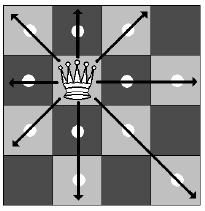
\includegraphics{docs/reina_movimientos.jpg}
  \caption{Movimientos posibles de una reina en un juego de Ajedréz}
\end{figure}

  Una solución posible puede escribirse de la siguiente manera con un vector
  solución (1,5,8,6,3,7,2,4). Éste mismo significa que se pueden ubicar las
  reinas en las siguientes posiciones definidas por el binomio (fila, columna)
\begin{lstlisting}
  (1, 1) : fila 1, columna 1
  (2, 5) : fila 2, columna 5
  (3, 8) : fila 3, columna 8
  (4, 6) : fila 4, columna 6
  (5, 3) : fila 5, columna 3
  (6, 7) : fila 6, columna 7
  (7, 2) : fila 7, columna 2 
  (8, 4) : fila 8, columna 4 
\end{lstlisting}
  Las reinas no son amenazadas entre ellas mismas con sus movimientos 
  (ver Figura~\ref{fig:ejemplo1}).
  
\begin{figure}[h!]
  \centering
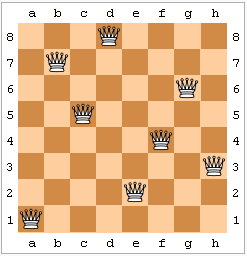
\includegraphics{docs/example_solution_15863724.png}
  \caption{Representación de la solución (1,5,8,6,3,7,2,4)}
  \label{fig:ejemplo1}
\end{figure}

\FloatBarrier

\section{Conclusiones}

  El problema de las ocho reinas tiene 92 soluciones, de las cuales 12 son 
  esencialmente distintas, es decir las 92 soluciones existentes se pueden 
  obtener a partir de simetrías, rotaciones y traslaciones de las 12 soluciones 
  únicas.

\clearpage

\part{Apendice}
\appendix

\section{Enunciado original}\label{sec:enunciado}
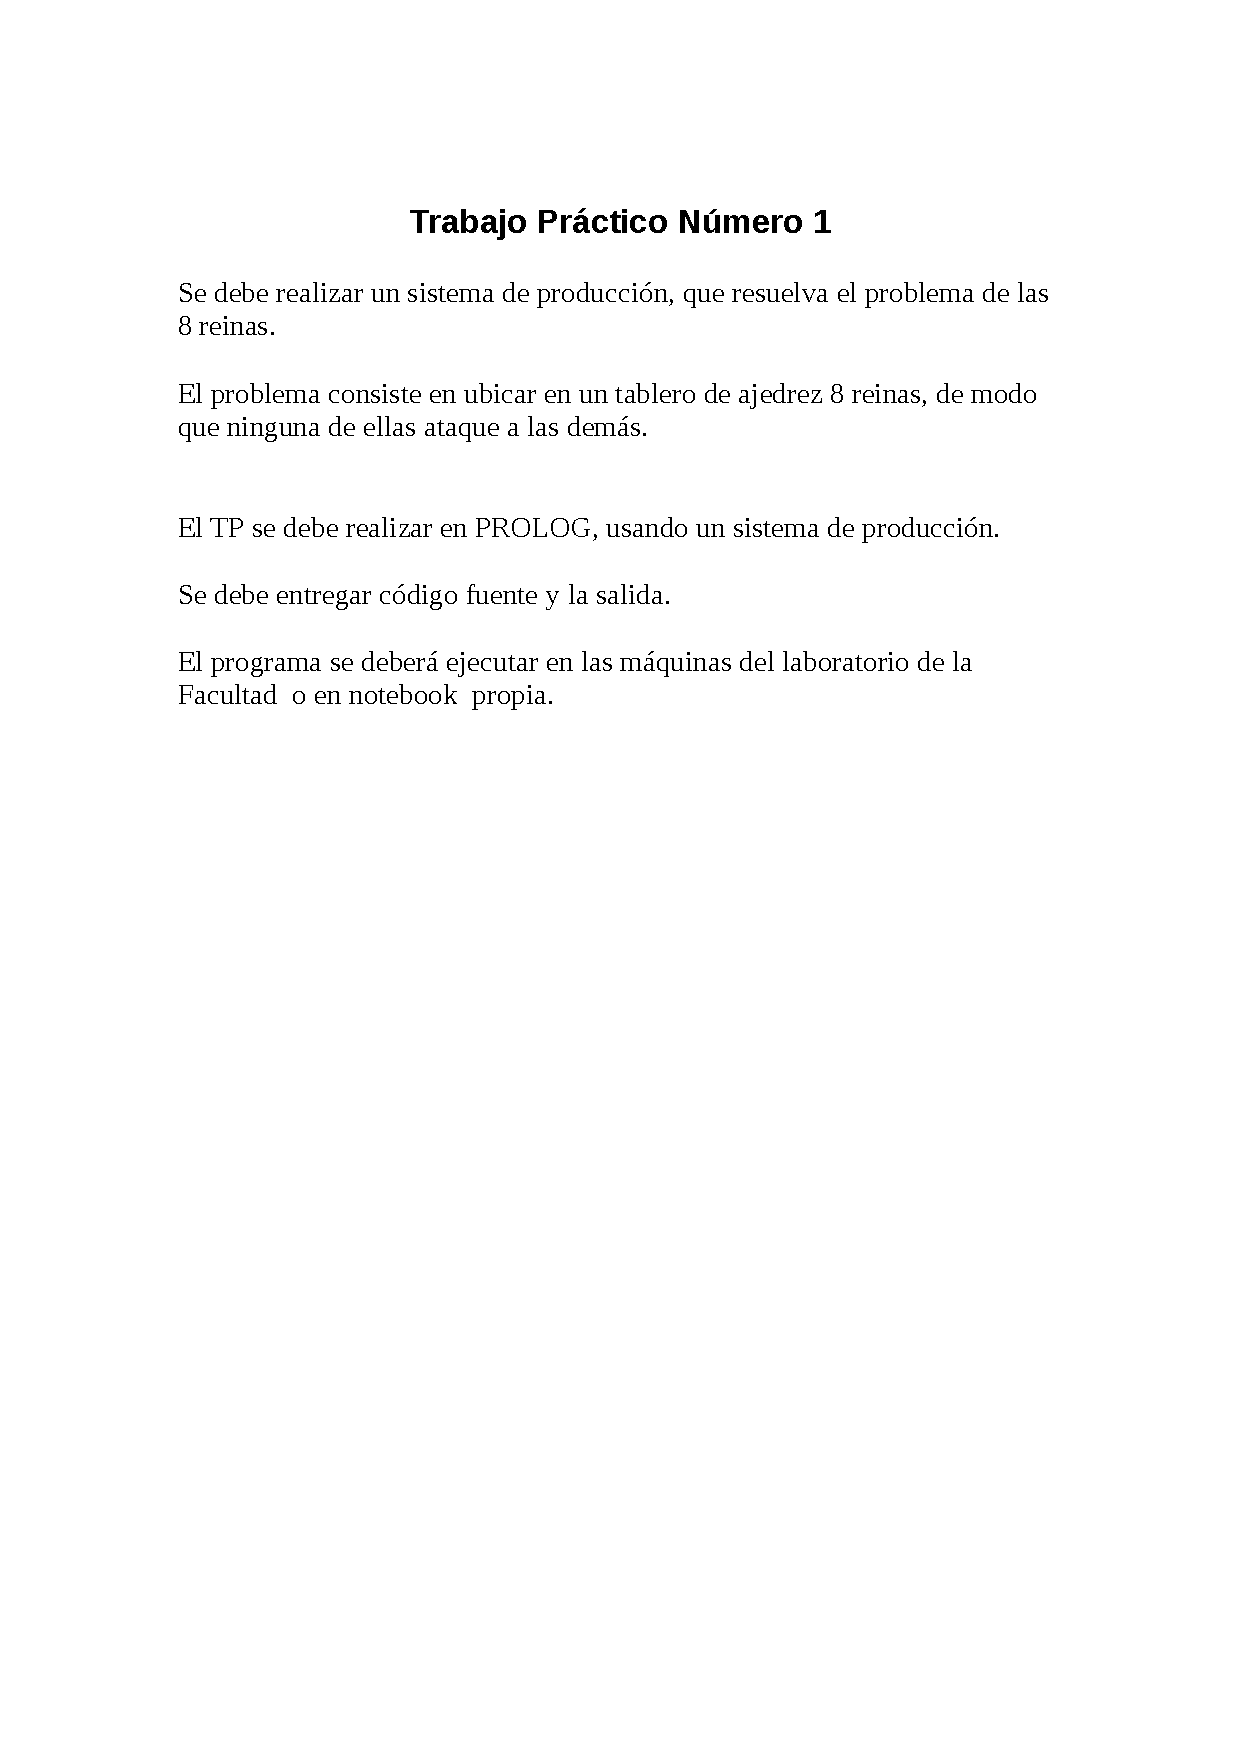
\includepdf[pages={-}]{docs/enunciado.pdf}

\clearpage
\section{Codigo fuente}\label{sec:source}
\clearpage
\definecolor{gray}{rgb}{0.5,0.5,0.5}
\lstset{%
  title=\lstname,
  language=Prolog,
  basicstyle=\footnotesize,
  showspaces=false,
  showstringspaces=false,
  breaklines=true,
  commentstyle=\color{blue},
  numbers=left,
  numberstyle=\tiny\color{gray},
  numbersep=5pt,
  frame=single
  unicode
}

\lstinputlisting{source/8reinas.pro}

\clearpage
\section{Soluciones}\label{sec:source}

Mostrando las 92 Soluciones:
\lstinputlisting{docs/soluciones.txt}

\end{document}
